\subsection{Communication}

I \textbf{communication diagram}, in maniera simile agli \textit{state diagram}, mostrano il funzionamento collettivo di un gruppo di partecipanti. L'enfasi è posta sui \textbf{messaggi scambiati} (non sul ciclo di vita) e sulle attività svolte da ciascun partecipante.

\paragraph{Partecipante} È un'\textbf{entità del dominio applicativo} nella \textit{prospettiva concettuale}, un \textbf{oggetto} nella \textit{prospettiva software}. Rappresentato da box con angoli smussati. I box sono collegati da linee continue, le quali possono:
\begin{itemize}
    \item tradurre associazioni statiche (tra partecipanti, \textit{compile-time})
    \item introdurre associazioni dinamiche (tra partecipanti, nascono e muoiono a \textit{run-time})
\end{itemize}

\paragraph{Messaggio} Rappresentato da frecce etichettate con l'azione corrispondente e numerato in maniera nidificata. Si usa:
\begin{itemize}
    \item $\langle\langle$create$\rangle\rangle$ per la creazione di partecipanti
    \item $\langle\langle$delete$\rangle\rangle$ per la distruzione di partecipanti
\end{itemize}
Inoltre, è possibile inserire lettere nelle etichette per indicare il thread che esegue l'operazione.

\begin{figure}[H]
    \centering
    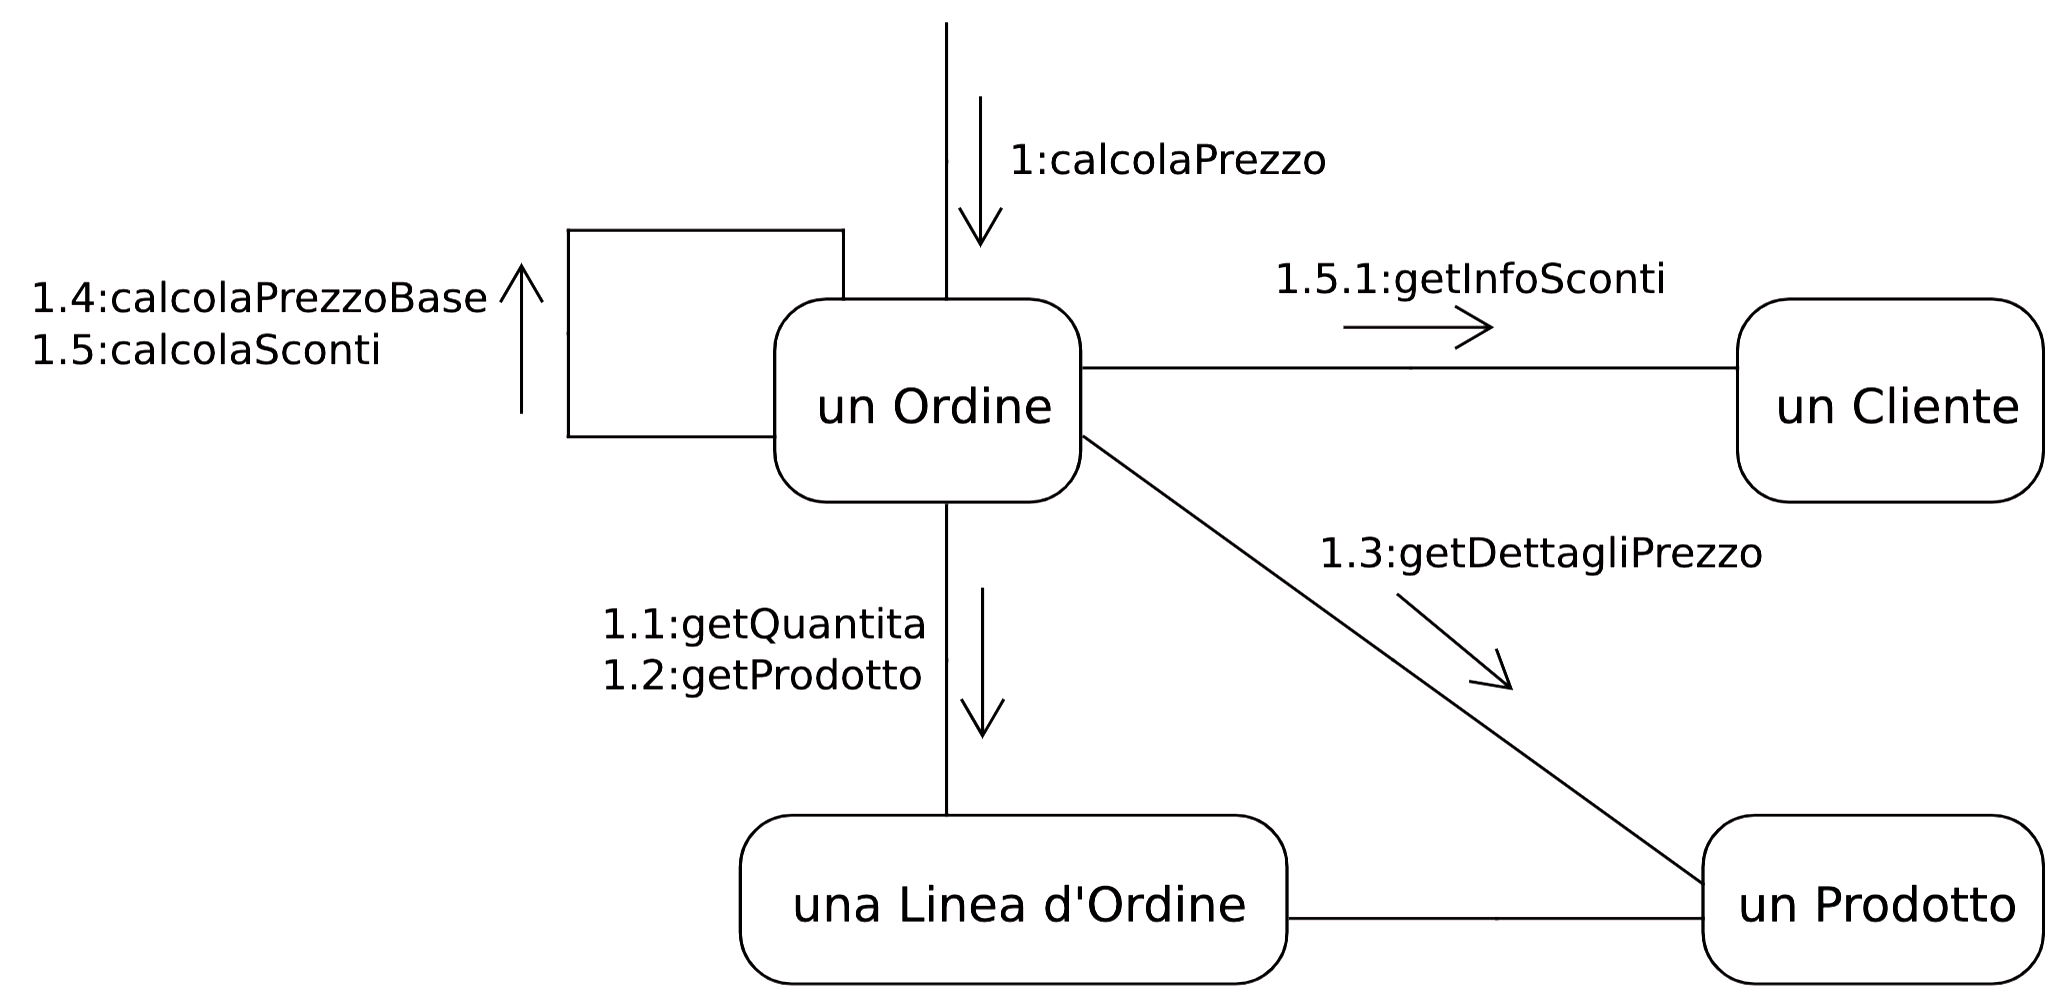
\includegraphics[width=0.75\linewidth]{assets/UML/communication/communication-1.png}
    \caption{Esempio di communication diagram a \textit{controllo centralizzato}.}
\end{figure}

\newpage